\section{Evaluation}
\label{sec:eval}

We deploy our GPU code on a consumer Nvidia GeForce GTX 1060\footnote{We use the Driver Version 572.42 and CUDA Toolkit 12.8 inside WSL2 (Ubuntu 22.04 jammy).} with 6GB GDDR5. Every code change related to the GPU code is verified by comparing the resulting binary edge weights file with the one generated by our parallelized Rust implementation on the CPU. This baseline helps to quickly identify errors, which could otherwise remain unnoticed. During our tests, we define a manual threshold to cap the number of words to a user-defined threshold. The words considered are sorted according to their frequency as we are interested in relationships between the most commonly used words.

\textbf{Performance.} A fair comparison between the CPU and GPU implementation is not possible since focus was put in optimizing the GPU code. For example, the CPU implementation currently stores the row and column number alongside the actual edge weight in RAM to be able to order the results to the row-major ordering afterwards. To give an order of magnitude, the parallelized Rust CPU implementation (without the subsequent sorting) takes around $\qty{12}{\s}$ (for 10,000 nodes), \qty{42}{\s} (for 20,000 nodes) and \qty{93}{\s} for 30,000 nodes on a 4-core Intel i7-6700 CPU. The implementation is limited to around 35,000 words when $\approx\qty{20}{\giga\byte}$ of RAM are available.

\begin{figure}[H]
    \centering
    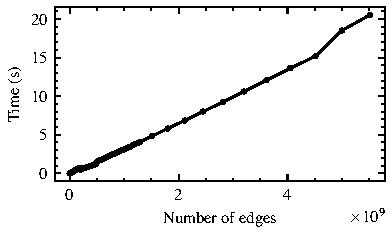
\includegraphics[width=\linewidth]{assets/timing.pdf}
    \caption{Performance of the GPU code for different number of nodes $n$. Number of edges via \eqref{eq:num-edges}.}
    \label{fig:timing}
\end{figure}

\vspace{-1.5em}

To test the performance of the GPU code, we measure the kernel execution time (including copying the results back to the host) for a range of number of nodes $n$ in the graph. For every $n$, we measure the duration 12 times\footnote{After every run, the device is re-initialized. Furthermore, we wait \qty{2}{\s} after every run before a new one starts.} and calculate mean and variance. The results are depicted in \autoref{fig:timing}. The variance is not shown as it is too small to be visible (always less than \qty{1}{\ms}). For $20,000$ words, the GPU code takes $\qty{484}{\ms}$ on average, while the CPU implementation needs $\qty{42}{\s}$. Up to $100,000$ nodes (\ie up to almost 5 billion edges), the GPU implementation takes less than \qty{20}{\s}. \autoref{fig:timing} also reveals the linear trend of time with increasing number of edges, which was to be expected since a thread is launched for every edge.

Our CUDA implementation is limited by the global memory (\qty{6}{\giga\byte} for the GPU at hand). This memory is used to store the resulting edge weights, \ie one byte per edge. The maximum number of edges we can handle is therefore the available memory divided by 1~byte. To obtain the corresponding number of nodes, we solve \eqref{eq:num-edges} for~$n$:
\begin{align}
    n = \frac{1}{2} + \sqrt{\frac{1}{4} + 2 \cdot \text{num edges}}
\end{align}
On the GPU at hand, we can handle up to around 107,000 nodes (mean time $\approx \qty{21.3}{\s}$) before experiencing \q{CUDA out of memory errors}. Currently we detect the limit, but do not implement a mechanism to go beyond it. One way could to be to detect the error, then copy the results back to the host and continue the computation while shifting the index back to $0$. The results are then concatenated on the host. For the further evaluation, we shall content ourselves with the results for the first 100,000 words, which already contain a lot of information of the French language. The binary file holding only the edge weights in row-major order, is \qty{4.66}{\giga\byte} in size.

\textbf{Graph application.} \autoref{fig:hist} shows the histogram of edge weights. It strongly resembles a normal distribution, which is probably due to how word lengths are distributed in the language. Note that the minimum and maximum achievable alignment score for a word pair depends on the word lengths. To efface this dependency, we normalize every score by dividing by $\max(\text{len}(A), \text{len}(B))$ and then multiply by 100. The resulting histogram is shown in \autoref{fig:hist-norm}. It does not resemble a normal distribution anymore. Most nodes have the smallest score of $-100$. There is a gap of around width 10 around edge weight 0 that we have no explanation for. The global trend is that many edges have a strong negative edge weight, while a smaller proportion have a strongly positive one.\label{paragraph:normalization}

The binary edge file is converted to a CSV file and imported into the open-source graph visualization software \href{https://gephi.org/}{Gephi}. As Gephi is far from being able to display 5 billion edges at the same time (let alone import such a file), we have to select specific ranges of edge weights we are interested in. We focus on the positive edge weights as they indicate a higher similarity between words.

Gephi implements various force-directed graph drawing algorithms that can help us gain a better understanding of the data. The principle of these algorithms is that nodes repulse each other, while edges act as springs to pull connected nodes together (taking into account the edge weights). Here, we exclusively use the algorithm by Yifan Hu\footnote{\href{http://yifanhu.net/PUB/graph_draw_small.pdf}{Efficient and High Quality Force-Directed Graph Drawing} by Yifan Hu in 2006.} as we found it to be the most efficient and reliable for our data. Furthermore, we run a modularity analysis using the Louvain method\footnote{\href{https://arxiv.org/abs/0803.0476}{Fast unfolding of communities in large networks} by Vincent Blondel et al.} implemented in Gephi. This method is used to detect communities in the graph, \ie groups of nodes that are more connected to each other than to the rest of the graph. We color the nodes according to the community they belong to (colors don't match between \textit{different} graphs in the following).

% \vfill\null

\begin{figure}[H]
    \centering
    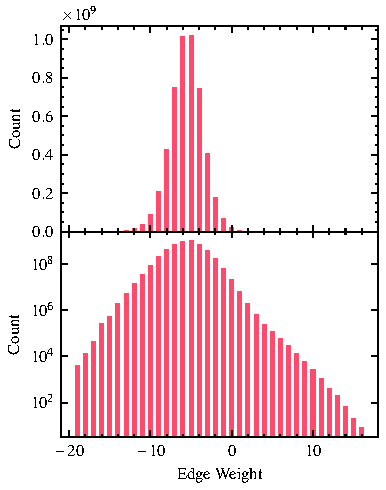
\includegraphics[width=\linewidth]{assets/edge_weights.pdf}
    \caption{Histogram of edge weights (linear and logarithmic scale). Mean: $-1.5$, range: $[-19, 16]$.}
    \label{fig:hist}
\end{figure}

% \vspace{-1em}

\begin{figure}[H]
    \centering
    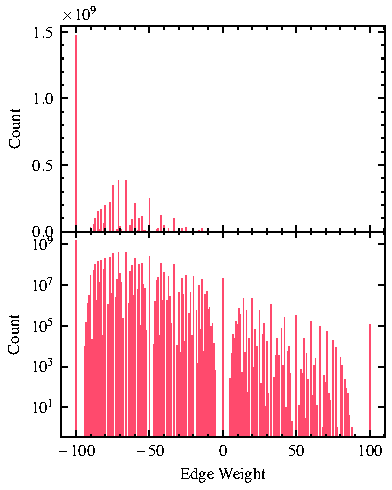
\includegraphics[width=\linewidth]{assets/edge_weights-normalized.pdf}
    \caption{Histogram of normalized edge weights. Linear and logarithmic scale.}
    \label{fig:hist-norm}
\end{figure}

\vfill\null
\columnbreak

\begin{figure*}[t]
    \centering
    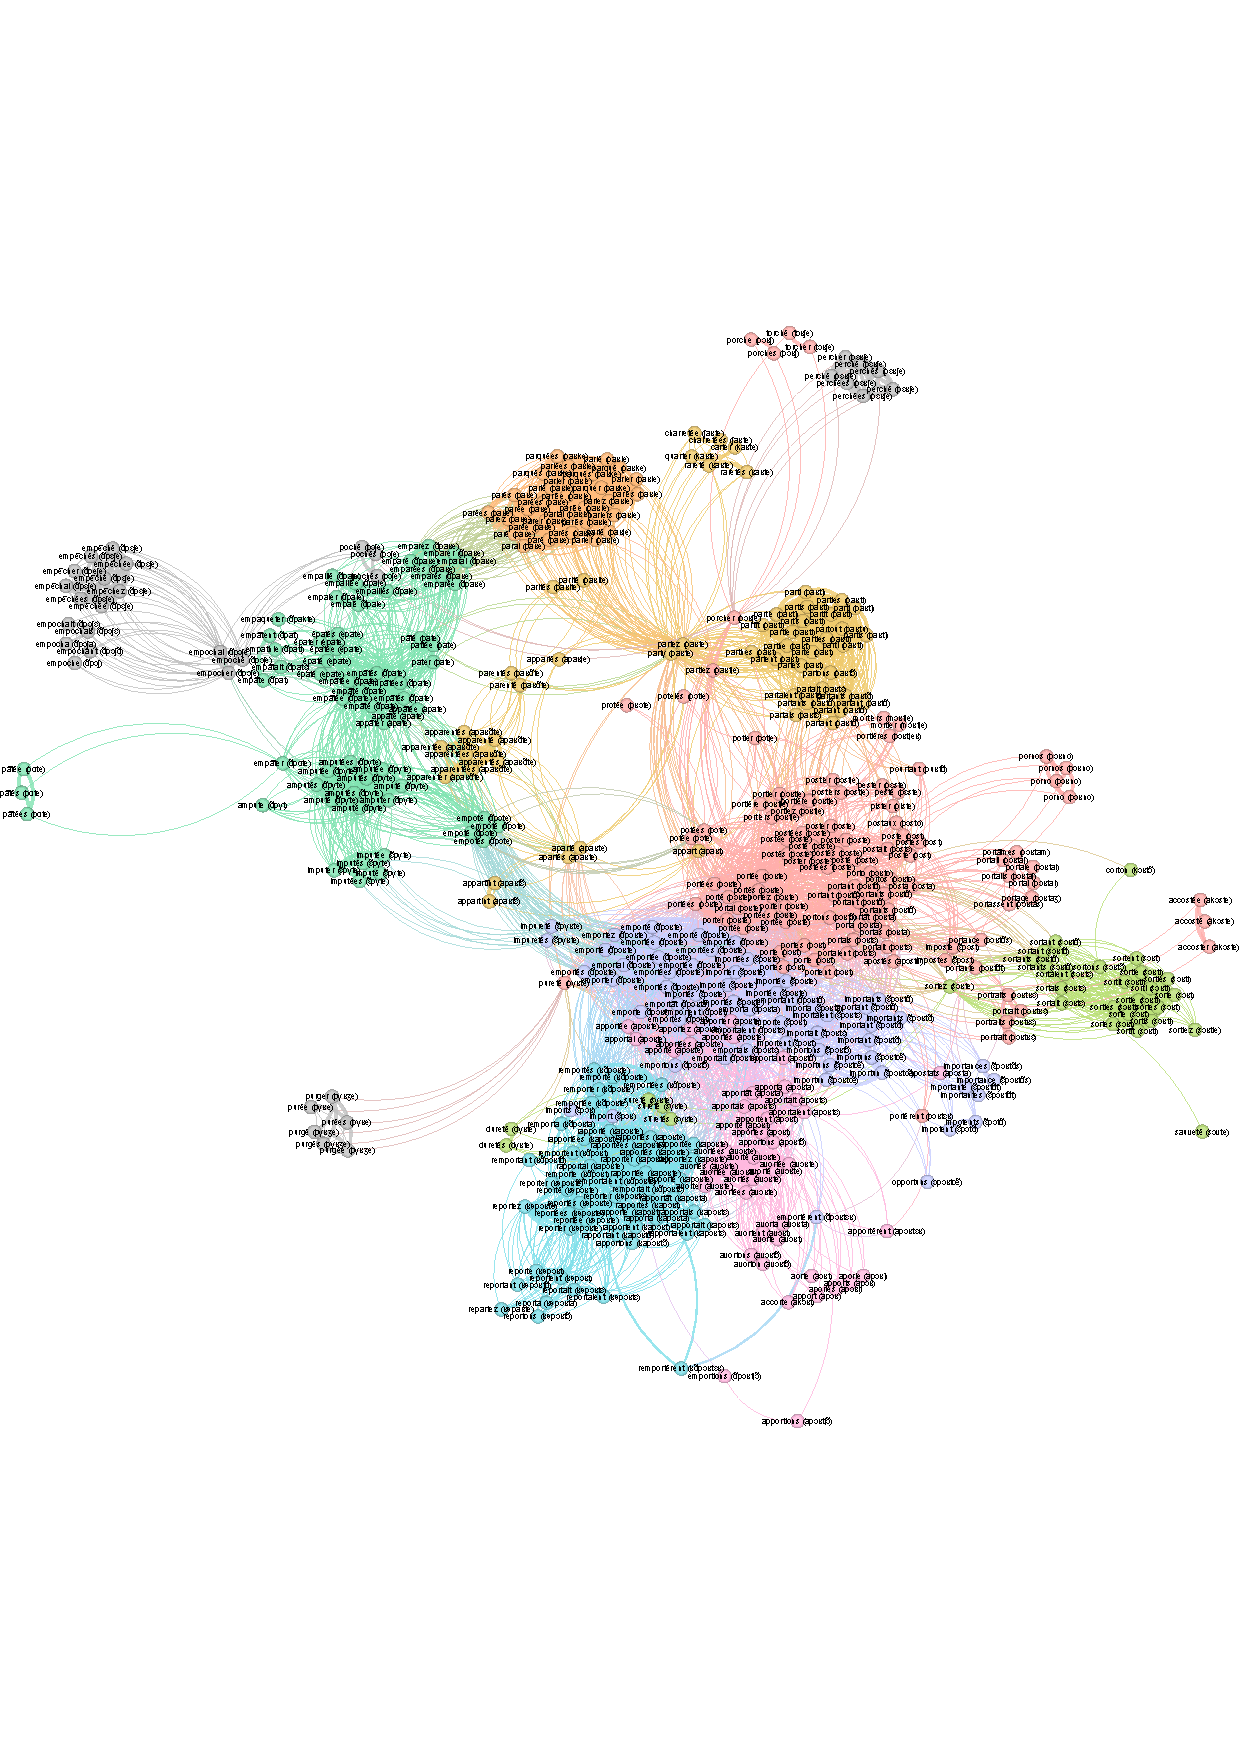
\includegraphics[width=\textwidth, trim=0cm 5.5cm 0cm 5.5cm, clip]{assets/emporter-ego.pdf}
    \caption{Ego-network (depth 3) of the word \textit{emporter} (to take away) for edge weights in the range $[60,100]$. This subgraph contains 449 nodes and 5921 edges.}
    \label{fig:emporter-ego}
\end{figure*}

\begin{figure}[H]
    \centering
    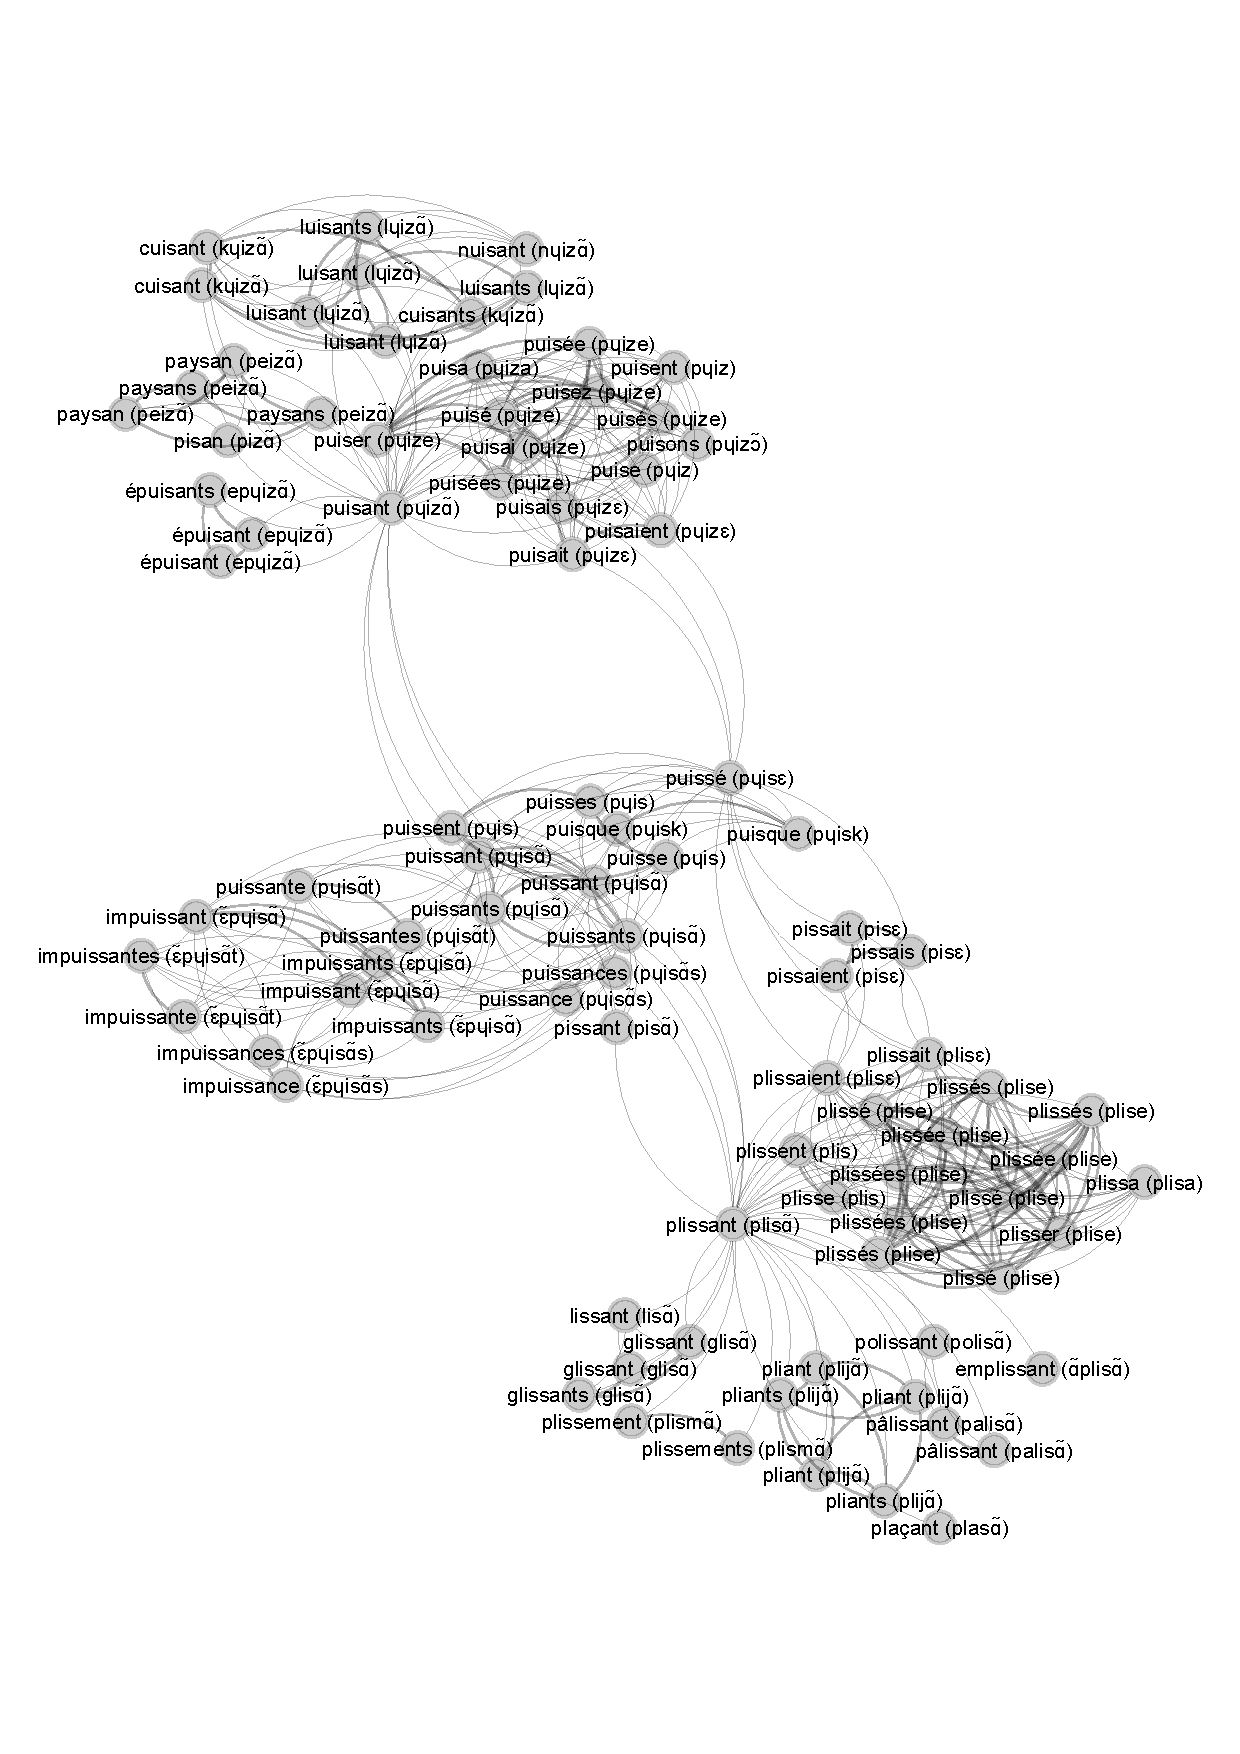
\includegraphics[width=\linewidth, trim=1cm 3.4cm 0.5cm 3.2cm, clip]{assets/puissant-ego.pdf}
    \caption{Ego-network (depth 3) of the word \textit{puissant}.}
    \label{fig:puissant-ego}
\end{figure}

\begin{figure}[H]
    \centering
    \includegraphics[width=\linewidth, trim=1cm 4.8cm 0.5cm 3.2cm, clip]{assets/étirer.pdf}
    \caption{Ego-network (depth 3) of the word \textit{étirer} for edge weights in the range $[40,49]$.}
    \label{fig:etirer-ego}
\end{figure}

Some resulting ego-networks are shown in figures \ref{fig:emporter-ego}, \ref{fig:puissant-ego} and \ref{fig:etirer-ego}. These graphs are constructed by locating neighbors of a word, then finding the neighbors of these neighbors up to a depth of~3. Different slices of edge weights are used, \eg in \autoref{fig:emporter-ego}, we have filtered the graph for edge weights in the range $[60,100]$ beforehand, which account for a total of 458,529 edges. The networks clearly show that our implementation is working correctly and that Needleman-Wunsch indeed gives a meaningful metric in this context.

\begin{itemize}[leftmargin=0cm]
    \item Words with the same pronunciation are as close as possible to each other and reside in the same community. In \autoref{fig:etirer-ego}, the words \textit{étudier}, \textit{étudient}, \textit{étudié}, \textit{étudiai}, \textit{étudiées} etc. are close to each other. In \autoref{fig:emporter-ego}, inside the red group in the middle-right part, we find different adjective endings for the word \textit{porté} (corresponding to gender and number of the noun it describes, \ie adjective agreement): porté, portée, portés, portées. We also find the words \textit{porter} and \textit{portez} here with the same prononciation as \textit{porté}. Note that it is claimed that \textit{portai} has the exact same prononciation, which is not correct (the last phoneme is different). This also shows that the dataset itself is not perfect and may contain errors. 
    
    \item Of greater interest are similar sounding words; as hoped for, they are close to each other in the graph. For example, in \autoref{fig:emporter-ego}, we find edges like \textit{emporté} -- \textit{porter}, \textit{emporté} -- \textit{importé}, \textit{importé} -- \textit{impureté} and \textit{impureté -- pureté}. It is also remarkable that words in one group almost exclusively start with the same letter and correspond to the same word root: \textit{sortir} in the green group on the right, \textit{porter} and \textit{poster} in the red group, \textit{emporter} and \textit{importer} in the violet group, \textit{apporter} in the rose group, \textit{rapporter}, \textit{reporter} and \textit{remporter} in the blue group etc.
    
    \item There are stronger and weaker connections between words. In \autoref{fig:puissant-ego}, the edge between \textit{puisant}\footnote{Note that this is not missing an additional \textit{s}. This is the word in a phrase like \q{en \textit{puisant} de l'eau, ...}.} -- \textit{épuisant} has weight $\nicefrac{200}{3}\approx 66.7$ (after normalization), while that of \textit{puisant} -- \textit{paysans} has the smaller weight $\nicefrac{300}{5} = 60$.
    \begin{table}[H]
        \centering
        \begin{tabular}{l*{6}{>{\centering\arraybackslash}p{0.2cm}}}
            \toprule
            \textit{paysans}
            & & \textipa{p} & \textipa{e} & \textipa{i} & \textipa{z} & \textipa{A}\\
            \midrule
            \textit{puisant}
            & & \textipa{p} & \textipa{\textturnh} & \textipa{i} & \textipa{z} & \textipa{\~A}\\
            \midrule
            \textit{épuisant}
            & \textipa{e} & \textipa{p} & \textipa{\textturnh} & \textipa{i} & \textipa{z} & \textipa{\~A}\\
            \bottomrule
        \end{tabular}
        \caption{Optimal alignment of three words.}
        \label{tab:align-puisant}
    \end{table}
    \vspace{-1.3em}

    \autoref{tab:align-puisant} shows the corresponding optimal alignments. With a match score of $1$, a mismatch score of $-1$ and a gap penalty $p=-1$, we find a score of~3 (\textit{puisant} -- \textit{paysans}) and 4 (\textit{puisant} -- \textit{épuisant}). With the normalization discussed on \autopageref{paragraph:normalization}, we indeed obtain the aforementioned edge weights. This example also illustrates that fine-tuning match/mismatch score and gap penalty is important to obtain meaningful results. One might want a greater distance between \textit{paysans} and \textit{puisant} since the \textipa{/u/} is replaced by the very different sounding \textipa{/a/}. Furthermore, the match/mismatch scores can be adjusted for every pair of phonemes to reflect the subtleties of a language. This can be done by changing the coefficients in the similarity matrix (see \autoref{algstep:sim} of \autoref{alg:needleman-wunsch}). In this document, we limit ourselves to the default scoring matrix ($1$ on the diagonals, $-1$ elsewhere).
\end{itemize}

\vspace{-1em}

\begin{figure}[H]
    \centering
    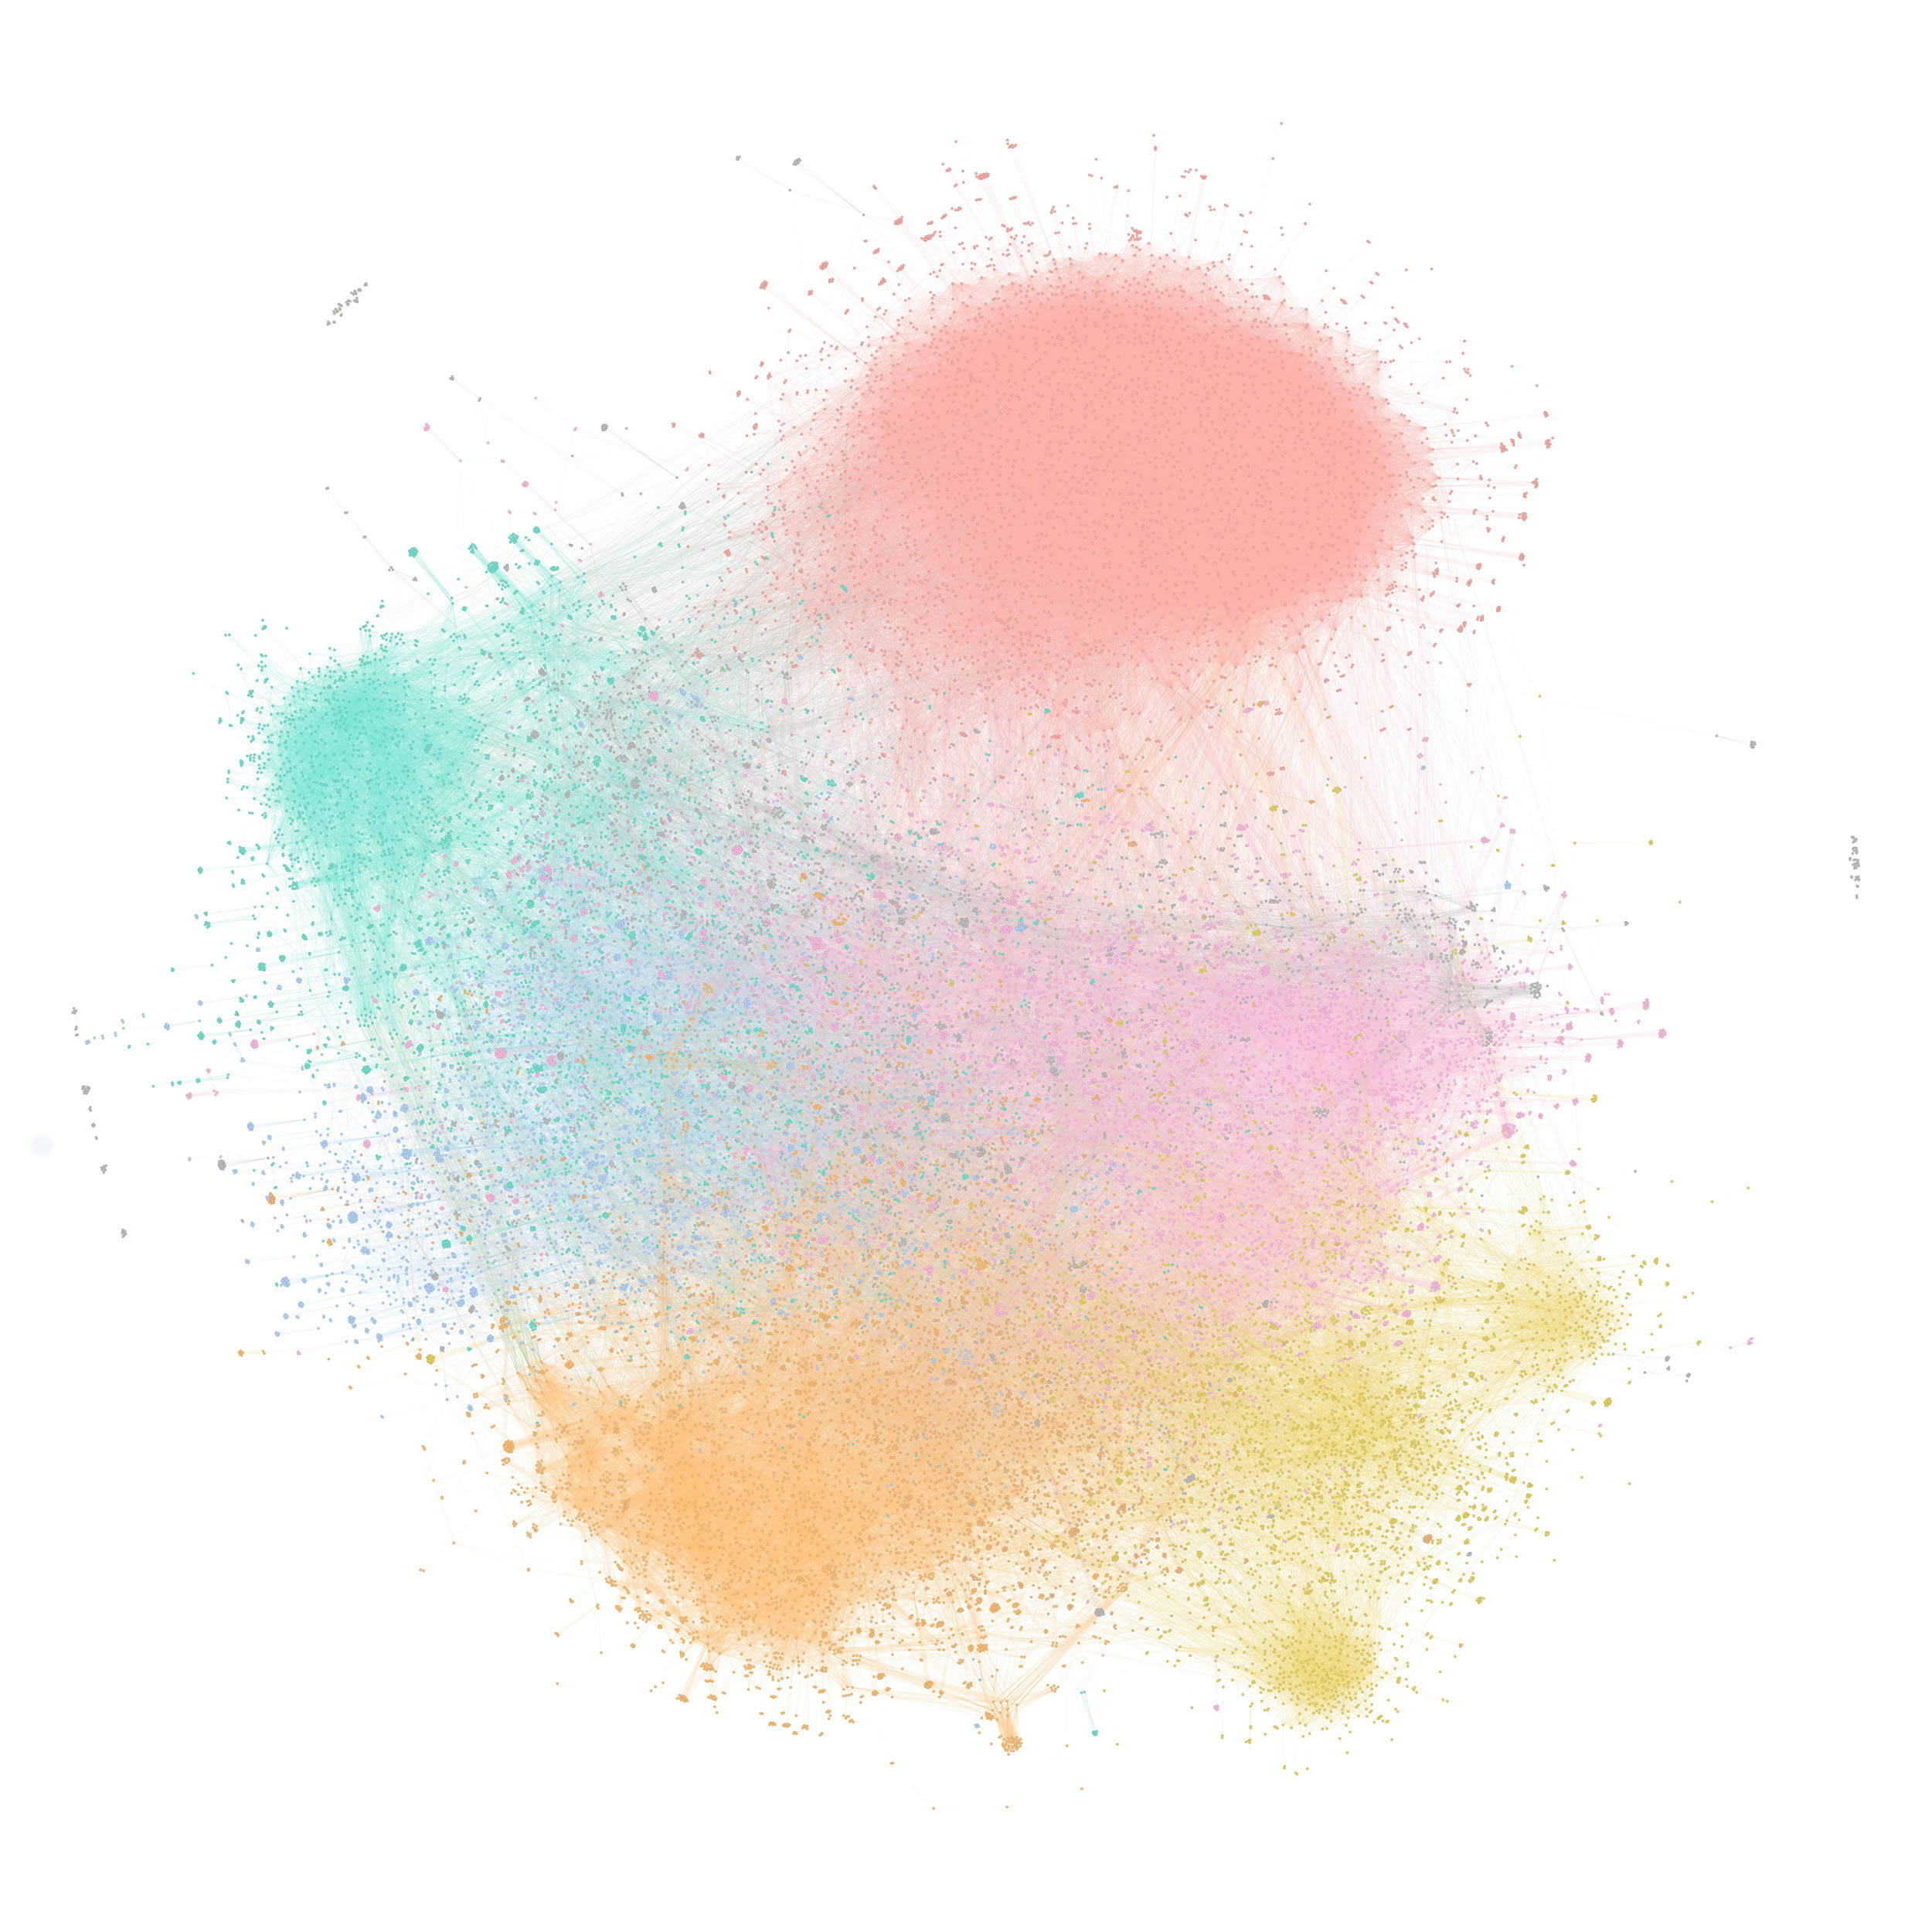
\includegraphics[width=0.9\linewidth, trim=1cm 4.8cm 0.5cm 3.2cm, clip]{assets/big view-min-min.jpg}
    \caption{Overview of the graph containing edge weights in the range $[8,10]$. 30,185 nodes and 306,473 edges are shown.}
    \label{fig:big-view}
\end{figure}

\vspace{-1.5em}

To broaden the view, we consider a bigger graph in \autoref{fig:big-view}, with normalized edge weights 8, 9 or 10. Communities found with Louvain are again color-coded. This very tiny slice of edge weights (compare \autoref{fig:hist-norm}) can already reveal interesting partitions of a language.

\begin{itemize}
    \item The red community at the top consists almost exclusively of words ending in \textipa{/j\~O/}, \eg \textit{illustration}, \textit{proportions}, \textit{réalisation}, \textit{fluctuation}, \textit{documentation}, \textit{émancipation}, \textit{articulation} etc.
    
    \item Below, the rose group encompasses words that end with \textipa{/\OE K/}, \eg \textit{aspirateur}, \textit{consommateur}, \textit{illustrateur}, \textit{radiateur}. However, this group is less homogeneous and also contains words ending in \textipa{/ktiv/}, \eg \textit{interactives}, \textit{réparatrice}, \textit{instructif}, \textit{instinctives}. 
    
    \item The orange group on the bottom mainly comprises words ending in \textit{e}, \eg \textit{personnalité}, \textit{caractérisé}, \textit{centraliser}, \textit{hospitalité}, \textit{réalité}, \textit{vivacité}, \textit{patienter}, \textit{spécialiser}, \textit{sensibiliser}, \textit{modéliser}.
    
    \item In the cyan group on the far left, we find many words that end in \textipa{El}, \eg \textit{personnel}, \textit{conventionnel}, \textit{professionnel}, \textit{conditionnelles}, \textit{exceptionnelle}, \textit{émotionnels}, \textit{sensationnels}. However, this group is harder to describe since it also contains different words like \textit{occasionnant}, \textit{collectionneur}, \textit{frictionne}, \textit{crayonné}, \textit{positionnement}.
    
    \item The yellow group on the bottom right is easier to classify: it contains words ending in \textipa{Zi} or \textipa{Zik}. Among others: \textit{méthodologique}, \textit{topologique} et \textit{topologie}, \textit{holistique}, \textit{diplomatique}, \textit{dramaturgie}, \textit{gastronomie}, \textit{cytologie}, \textit{phénoménologie}, \textit{biologie}, \textit{écologique}, \textit{synchronique}. 
\end{itemize}

We also tried to identify common groups of words \textit{between} two communities in the expectation of finding a \q{morphing} behavior between them. However, this could not be observed in the graphs and we were not able to find a meaningful way to group these words.

Finally, having translated the problem into a graph structure also allows us to use graph algorithms to discover interesting properties. As an example, Gephi implements the \textit{shortest path algorithm}: users can click on two words and the shortest path between them is calculated and shown in the graph. Beforehand, we filtered the graph to only include the most strong edges. With this, we can find chains like the following (read them aloud to hear the phonetic similarity):
\begin{itemize}
    \item trottoir $\rightarrow$ entrevoir $\rightarrow$ devoir $\rightarrow$ voire $\rightarrow$ voile $\rightarrow$ val $\rightarrow$ valait $\rightarrow$ fallait $\rightarrow$ falaise
    \item falaise $\rightarrow$ fallait $\rightarrow$ palais $\rightarrow$ passais $\rightarrow$ dépassait $\rightarrow$ dépendait $\rightarrow$ répondait $\rightarrow$ répond $\rightarrow$ raison $\rightarrow$ maison
    \item confusion $\rightarrow$ conclusion $\rightarrow$ exclusion $\rightarrow$ explosion $\rightarrow$ exposition $\rightarrow$ explications $\rightarrow$ respiration $\rightarrow$ précipitation $\rightarrow$ présentation $\rightarrow$ présenta $\rightarrow$ présente $\rightarrow$ présence $\rightarrow$ présidence $\rightarrow$ résidence $\rightarrow$ résistance $\rightarrow$ existence
\end{itemize}
